\documentclass[output=paper]{langsci/langscibook} 
\author{%
Anthony Davis\affiliation{Buffalo?}%
\lastand Jean-Pierre Koenig\affiliation{University at Buffalo}%
}
\title{The nature and role of the lexicon in HPSG}

% \chapterDOI{} %will be filled in at production

%\epigram{Change epigram in chapters/03.tex or remove it there }
\abstract{This chapter discusses the critical role the lexicon plays in HPSG and the approach to lexical knowledge that is specific to HPSG.
We describe the tenets of lexicalism in general, and discuss the nature and content of lexical entries in HPSG.
As a lexicalist theory, HPSG treat lexical entries as informationally rich, representing the combinatorial properties of words as well as their part of speech, phonology, and semantics.
Thus many phenomena receive a lexically-based account, including some that go beyond what is typically regarded as lexical.
We then turn to the global structure of the HPSG lexicon, the hierarchical lexicon and inheritance.
We show how the extensive type hierarchy employed in HPSG accounts for lexical generalizations at various levels and discuss some of the advantages of default (nonmonotonic) inheritance over simple monotonic inheritance.
We then describe lexical rules and their various proposed uses in HPSG, comparing them to
alternative approaches to relate lexemes and words based on the same root or stem.}

\maketitle

\begin{document}
\label{chap-lexicon}

\avmoptions{center}

\section{Introduction}

The nature, structure, and role of the lexicon in the grammar of natural languages has been a subject of debate for at least the last 50 years. For some, the lexicon is a prison that ``contains only the lawless''  to borrow a memorable phrase from \citew{DiSciulloandWilliams1987}, and not much of interest resides there. In some recent views, the lexicon records merely phonological information and some world knowledge about each lexical entry (see \citet{Marantz1997}). All of the action is in the syntax, save the expression of complex syntactic objects as inflected words.
In contrast, lexicalist theories of grammar, and HPSG in particular, posit a rich and complex lexicon embodying much of grammatical knowledge.

This chapter has two principal goals.  One is to review the arguments for and against a lexicalist view of grammar within the generative tradition.  The other is to survey the HPSG implementation of lexicalism. In regard to the first goal, we begin with the reaction to Generative Semantics, and note developments that led to lexicalist theories of grammar such as LFG and then HPSG.  Central to these developments was the argument that lexical processes, rather than transformational ones, provided more perspicuous accounts of derivational morphological processes.  The same kinds of arguments then naturally extended to phenomena like passivization, which had previously been treated as syntactic.  Once on this path, lexical treatments of other prototypically syntactic phenomena — long distance extraction, \word{wh}-movement, word order, and anaphoric binding — were advanced as well, with HPSG playing a leading role.

But this does not mean that opposition to lexicalism melted away.  Both Minimalism (cross-ref here), in particular Distributed Morphology, and Construction Grammar (cross-ref here) claim that lexicalist accounts fail in various ways.  We discuss some of these current issues, including phrasal processes in the lexicon, word-internal ellipsis, and endoclitics, each of which poses challenges for those who advocate a strict separation between lexical and syntactic systems.  While we maintain that the anti-lexicalist arguments are not especially strong, and the phenomena they are based somewhat marginal, we acknowledge that these questions are not yet settled. We then turn to the specifics of the lexicon as modeled within HPSG.  Lexicalism demands, of course, that lexical entries be informationally rich, encoding not merely idiosyncratic properties of a single lexical item like its phonology and semantics, but also more general characteristics like its combinatorial possibilities.  We outline what HPSG lexical entries must contain, and how that information is represented.  This leads naturally to the next topic: with so much information in a lexical entry, and so much of that repeated in similar ones, how is massive redundancy avoided?  The hierarchical lexicon, in which individual lexical entries are the leaves of a multiple inheritance hierarchy, is a core component of HPSG.  Types throughout the hierarchy capture information common to classes of lexical entries, thereby allowing researchers to express generalizations at various levels.  Just as all verbs share certain properties, all transitive verbs, all verbs of caused motion, and all transitive verbs of caused motion share additional properties, represented as constraints on types within the hierarchy.  We draw on examples from linking, gerunds, and passives as illustrations, but many others could be added.

Constraints specified on types in the hierarchy are deemed to be inherited by their subtypes, but monotonic inheritance of this kind runs into vexing issues.  Most obviously, there are irregular morphological forms; any attempt to represent, say, the phonology of English plurals, as a constraint on a plural noun class in the hierarchical lexicon must then explain why the plural of \word{child} is \word{children} and not *\word{childs}.  Beyond this simple example, there are ubiquitous cases of lexical generalizations that are true by default, but not always.  Various mechanisms for modeling default inheritance have therefore been one focus within HPSG, and we furnish an example of their use in modeling the properties of gerunds cross-linguistically.

Finally, we discuss lexical rules and their alternatives.  Along with the ``vertical'' relationships between classes of lexical entries modeled by types and their subtypes in the hierarchical lexicon, there is a perceived need for ``horizontal'' relationships between lexical entries that are based on a single root or stem, such as forms of inflectional paradigms.  Yet formalizing lexical rules adequately within HPSG has proven tricky; specifying just what information is preserved and what is changed by a lexical rule is one prominent issue.  We conclude this chapter by describing alternatives to lexical rules.  One is implicational statements on partially specified feature structures; this might be thought of as a kind of ``online lexical rule''.  The second augments the type hierarchy via online type construction, extending the predefined lexical types specified in the hierarchy to include ``virtual types'' that combine the information from multiple predefined types.


\section{Lexicalism}
\label{sec:lex}
\subsection{Lexicalism and the origins of HPSG}

Lexicalism began as a reaction to Generative Semantics, which treated any regularity in the structure of words (derivational patterns, broadly speaking) as only ephiphenomenally a matter of word structure and underlyingly as a matter of syntactic structure (see \citet{Lakoff1970}, among others). In the Generative Semantics view, all grammatical regularities are a matter of syntax (much of it, in fact, logical syntax). \citet{Chomsky1970} presented many arguments that lexical knowledge differs qualitatively from syntactic knowledge and should be modeled differently. \citet{Jackendoff75a} is an explicit model of lexical knowledge that follows Chomsky's insights, although it focuses exclusively on derivational morphological processes. The main insight that Jackendoff formalizes is that relations between stems and words (say, between \word{destruct} and \word{destruction}) are to be modeled not via a generative device but through a redundancy mechanism that measures the relative complexity of a lexicon where these relations are present or not present (the idea is that a lexicon where \word{construct} and \word{construction} are related is simpler than one where they are not). \citet{Bochner1993} is the most formalized and detailed version of this approach to lexical relations. Lexicalist approaches, including LFG and HPSG, took their lead from Jackendoff's work.  LFG relied heavily on treating relations between stems and between words as lexical rules, rather than the kind of generative devices that one finds in syntax. But, as accounts of linguistic phenomena in LFG focused increasingly on the lexicon, the question of whether lexical rules retained the character of redundancy rules or turned into yet another kind of generative device arose.  Consequently, the necessity of lexical rules has been questioned as well (see \citet{KoenigandJurafsky1994} and \citet{Koenig99a} for potential issues that arise once lexical rules are assumed to be involved in the creation of new lexical entries). 

Lexicalism, at least within HPSG, embodies two distinct ideas. First is the idea that parts of words are invisible to syntactic operations (\emph{lexical integrity}, see \citealt{BresnanandMchombo1995}), so that relations between stems and between word forms cannot be the result of or follow syntactic operations, as in distributed morphology, or other linguistic models that assign no special status to the notion of word. Relations between words are therefore not modeled via syntactic operations (hence the appeal to Jackendoff's lexical rules). Second is the idea that the occurrence of a lexical head in distinct syntactic contexts arises from distinct variants of words. For instance, the fact that the verb \word{expect} can occur both with a finite clause and an NP+VP sequence (see (\ref{expect-a}) vs. (\ref{expect-b})) means that there are two variants of the verb \word{expect}, one that subcategorizes for a finite clause and one where it subcategorizes for an NP+VP sequence.\footnote{As this chapter is an overview of the approach to lexical knowledge HPSG embodies rather than a description of particular HPSG analyses of phenomena, we will sample liberally from various illustrative examples and simplify whenever possible the analyses so that readers can see the forest and not get lost in the trees.} Not all lexicalist theories, though, cash out these two distinct ideas the same way. The net effect of lexicalism within HPSG is that words and phrases are put together via distinct sets of constructions and that words are syntactic atoms. These two assumptions justify positing two kinds of signs, \type{phrasal-sign} and \type{lexical-sign} and go hand in hand with the surface-oriented character of HPSG and what one might call a principle of surface combinatorics: If expression A consists of B$\oplus$C, then all grammatical constraints that make reference to B and C are circumscribed to A. 

\begin{exe}
	\ex \label{expect-a} I expected to leave yesterday
	\ex \label{expect-b} I expected that I would leave yesterday.
\end{exe}

An evident concern regarding this view of the lexicon is the potential proliferation of lexical entries, replete with redundant information. Will it be necessary to specify all the information in these two entries for \word{expect} without regard for the large amount of duplication between them? Will the same duplication be needed for the verb  \word{hope}, which patterns similarly? How will somewhat similar verbs, such as \word{imagine} and \word{suppose}, which allow finite complements but not infinitive ones, be represented? We will describe HPSG's solutions to these questions below, in our discussion of the hierarchical lexicon. First, however, we turn to recent arguments against lexicalism, and then discuss in more detail just what kinds of information should be in HPSG lexical entries.

\subsection{Recent challenges to lexicalism}

As there are been several challenges to lexicalism (see \citet{Bruening2018} and  \citet{Haspelmath2011} among others for some recent challenges), we now explore lexicalism and lexical integrity in HPSG in more detail. We first note that lexicalism does not imply that word and phrase formation are necessarily different ``components'' as is often claimed (see \citealt{Marantz1997}, \citet{Bruening2018}). Some lexicalist approaches \emph{do} assume that word formation and phrase building belong to two different components of a language's grammar (this is certainly true of \citealt{Jackendoff75a}), but they need not. Within HPSG, there are approaches that treat every sign-formation (be it word-internal or word-external) as resulting from typed mother-daughter configurations (this is the hypothesis pursued in \citew{Koenig99a}, and is also the approach frequently taken in implementations of large-scale grammars where lexical rules are modeled as unary-branching trees, see the English Resource Grammar at \url{http://www.delph-in.net/erg/}). Furthermore, recent approaches to inflectional morphology model realizational rules through the very same tools the rest of a language's grammar uses (see \citet{CrysmannandBonami2016} and the chapter on morphology in this volume).  There are also approaches to phrases where the same analytical tools developed to model lexical knowledge (see Section \ref{sec:hier-lex}) are employed to model phrase-structural constructions (see Sag's 1997 analysis of relative clauses, for example). So, both in terms of the formal devices and in terms of analytical tools used to model datasets, words and phrases can be treated the same way in HPSG (alhtough they need not be). Somewhat ironically, and despite claims to the contrary, word formation in the syntacticocentric approach Marantz or Bruening advocate \emph{does} make use of distinct formal machinery to model word formation, namely realizational rules to model inflectional morphology (see \citealt{HalleandMarantz1993}).

With this red herring out of the way, we concentrate on the two most important challenges \citet{Bruening2018} and \citet{Haspelmath2011} present to lexicalist views. The first challenge are cases of phrasal syntax feeding the lexicon, purportedly exemplified by sentences such as (\ref{bruen1}).

\begin{exe}
	\ex\label{bruen1} I gave her a don't-you-dare! look. (example (1a) in \citealt{Bruening2018})
\end{exe}

We can provisionally accept for the sake of argument Bruening's contention that \word{don't-you-dare!} is a word in (\ref{bruen1}), despite its reliance on the (unjustified) assumption that the secondary object in (\ref{bruen1}) involves N-N compounding rather than an AP N structure (we refer readers to \citet{BresnanandMchombo1995} or \citet{MuellerPersian} for counter-arguments to Bruening's claim). Crucially, though, examples such as (\ref{bruen1}) have no bearing on HPSG's model of lexical knowledge, as HPSG-style lexicalism does not preclude constructions that form words from phrases. Nothing, as far as we know, rules out constructions of the form \type{phrase} $\rightarrow$ \type{stem/word} in HPSG. The two assumptions underlying HPSG brand of lexicalism we mentioned above do not preclude a \type{lexical-sign} having a \type{phrasal-sign} as sole daughter (although we do not know of any HPSG work that exploits this possibility) and examples such as (\ref{bruen1}) are simply irrelevant to whether HPSG's lexicalist stance is empirically correct.

The second challenge to lexicalism presented in \citet{Bruening2018} bears more directly on HPSG's assumption that words are syntactic atoms. Word-internal conjunction/ellipsis examples, illustrated in (\ref{ch08}) (adapted from Bruening's (31a)), seem to violate the assumption that syntactic constraints cannot ``see'' the internal structure of words, as ellipsis in these kinds of examples seems to have access to the internal part of the word \word{over-application}. In fact, though, such examples do not violate lexical integrity if one enriches the representation of composite words (to borrow a term from \citealt{Anderson1992}) to include a representation of their internal phonological parts as proposed in \citet{Chaves2008,Chaves2014}.

\begin{exe}
	\ex\label{ch08}Over- and under-application of stress rules plagues Jim's analysis.
\end{exe} 

Chaves' analysis assumes that the phonology of compound words and words that contain affixoids (to borrom a term from \citealt{Booij2005}) is structured. The MorphoPhonology or \attrib{mp} attribute of words (and phrases) is a list of phonological forms and morphs information. The \attrib{mp} of compound words and words that contain affixoids includes a separate member for each member of the compound, or for the affixoid and stem.  Thus in (\ref{ch08}), the \attrib{mp}s of \word{overapplication} and \word{underapplication} each contain two elements: one for \word{over}/\word{under}, and one for \word{application}. Given this enriched representation of the morphophonology of words like \word{under/overapplication}, a single ellipsis rule can apply both to phrases and to composite words, eliding the second member of the word \word{overapplication}'s \attrib{mp}. As Chaves makes clear (p.304) such an analysis is fully compatible with lexical integrity, as there is no access to the internal structure of composite words, only to the (enriched) morphophonology of the entire word.

\citet{Haspelmath2011} similarly challenges the view that syntactic processes may not access the internal structure of words, although Haspelmath's point is merely that what is a word is cross-linguistically unclear. So-called suspended affixation in Turkish (see (\ref{turk})) also shows that word parts can be elided. We cannot discuss here whether Chaves' analysis can be extended to cases like (\ref{turk}) where suffixes are seemingly elided or whether lexical sharing (where a single word can be the daughter of two c-structure nodes \`a la \citealt{McCawley1982}), as proposed in \citet{Broadwell2008} is needed. What is important for current purposes is that these putative challenges to lexical integrity such as (\ref{ch08}) or (\ref{turk}) do not necessarily render a substantive version of it implausible. The same is true of another potential challenge to lexical integrity which neither Bruening nor Haspelmath discuss, endoclitics, which we discuss next.

\begin{exe}
	\ex\label{turk}
	\gll kedi ve köpek-ler-im-e \\
	cat and dog-\ig{pl-1sg-dat} \\
	\glt `to my cat(s) and dogs'	
\end{exe}


Endoclitics are clitics that at least appear to be situated within a word, rather than immediately preceding or following it, as clitics often do. (cross-reference to Abeill\'{e} \& Penn chapter on clitics)
In many cases, endoclitics appear at morphological boundaries, as in the well-studied pronominal clitics of European Portuguese \citep{Crysmann2000a}. An approach similar to what we have referenced above for composite words and elided morphology may well extend to these as well. But some trickier cases have also come to light, in which the clitic appears within a morpheme, not at a boundary. Two of the best documented cases from the Northeast Caucasian language Udi \citep{Harris2000} and from Pashto \citep{Tegey1977,Roberts2000,Dost2007}.
Here are examples from Udi (\ref{udi-endo}) and Pashto (\ref{pashto-endo}), where the clitics appear in the middle of verbs.

\begin{exe}
	\ex\label{udi-endo}
	\gll q'a\v{c}a\textipa{G}-\textipa{G}-on bez t\"{a}nginax ba\v{s}=\textbf{q'un}-q'-e \\
	thief-\ig{pl-erg} my money.\ig{dat} steal$_{1}$-\ig{3pl}-steal$_{2}$-\ig{aorII} \\
	\glt `Thieves stole my money.' (root \word{ba\v{s}q'}, 'steal')
\end{exe}


\begin{exe}
	\ex\label{pashto-endo}
	\begin{xlist}
		\ex\label{pashto-endo-a}
		\gll \textrtailt\textipa{@}lw\textipa{A}h\textipa{\'@}=\textbf{me} \\
		push.\ig{impf.pst.3sg}-cl.\ig{1sg} \\
		\glt 'I was pushing it.' (from \citealt{Tegey1977,Dost2007})
		\ex\label{pashto-endo-b}
		\gll \textrtailt\textipa{\'@}l=\textbf{me}-w\textipa{A}h\textipa{@} \\
		push$_{1}$-cl.\ig{1sg}-push$_{2}$.\ig{pf.pst.3sg} \\
		\glt `I pushed it.' (from \citealt{Tegey1977,Dost2007})
	\end{xlist}
\end{exe}

In these cases. as with clitics in general, there is a clash between the phonological criteria for wordhood, under which the clitics would be regarded as incorporated within words, and the syntactic constituency and semantic compositionality.
But what makes these particularly odd is that these clitics are situated word-internally, even morpheme-internally.
Udi subject agreement clitics such as \word{q'un} in (\ref{udi-endo}) typically attach to a focused constituent, which can be a noun, a questioned constituent, or a negation particle as well as a verb \citep{Harris2000}.
Under certain conditions, as in (\ref{udi-endo}), none of these options is available or permitted, and the clitic is inserted before the final consonant of the verb root, dividing it in two pieces, neither of which has any independent morphological status.
Its position in this instance is apparently phonologically determined; it cannot appear word-finally or word initially, and as there is no morphological boundary within the word it must therefore appear within the monomorphemic root.
Pashto clitics seek ``second position,'' whether at the phrasal, morphological, or phonological level; \word{me} in (\ref{pashto-endo}) appears to be situated after the first stressed syllable (or metrical foot), which, in the case of (\ref{pashto-endo-b}), also divides the verb into two parts that lack any independent morphological status.

If clitics are viewed as a syntactic phenomenon (``phrasal affixes'', as \citet{Anderson2005} puts it), these endoclitics must have ``visibility'' into the internal structure of words (be it morphological, prosodic, or something else), thereby seemingly violating lexical integrity. Anderson's brief account invokes a reranking of optimality theoretic constraints from their typical ordering, whereby the clitic's positional requirements outrank lexical integrity requirements. \citet{Crysmann2000b} proposes an analysis, paralleling in many respects his account of European Portuguese clitics in \citet{Crysmann2000a}, using Kathol's topological fields \citep{Kathol1999}. The ``morphosyntactic paradox in Udi'' is effectively ``resolved on the basis of discontinuous lexical items''; this account then ``parallels HPSG's representation of syntactic discontinuity.''  (cross reference to M\"{u}ller's chapter on word order here)

For Pashto, researchers generally agree that the notion of second position is crucial, but that it can be defined at various levels--- phrasal, lexical, and phonological. In this last case clitics can appear within a word following the first metrical unit, as illustrated above. (cross reference to Tseng's chapter on phonology, and Crysmann's on morphology here). \citet{Dost2007} invokes word order domains \citep{Reape1994} and topological fields \citep{Kathol1999} at these various levels to account for this distribution of clitics. In this analysis, some words contain more than one order domain at the prosodic level. Lexical integrity is preserved to the extent that, while domains at the prosodic level are ``visible'' to clitics in Pashto, syntatic processes do not reference the internal makeup of words.

Still, these accounts of endoclitics in Udi and Pashto appear to breach the wall of the strictest kind lexical integrity, requiring that they have access to some of the internal structure of lexical entries through a partial decomposition of their morphophonology into distinct order domains. Yet we would not wish to advocate models that permit unconstrained violations of lexical integrity, either. The troublesome cases we have noted here are relatively marginal or cross-linguistically rare, and limited in scope to prosodic or morphophonological information and seem to only pertain to phonological interactions (ellipsis, insertion). As \citet{Broadwell2008} points out when comparing possible analyses of Turkish suspended affixation, rejecting lexicalism altogether may lead to an unconstrained theory of the interaction between words/stems and phrases and incorrect predictions (e.g., that all affixes in Turkish can be suspended). Likewise, we would not expect to find a language in which endoclitics positioning is utterly unconstrained, and thus we would not wish to see grammatical theories abandon lexical integrity altogether.

\section{Lexical entries in HPSG}

\subsection{What are lexical entries?}

A consequence of HPSG's lexicalist stance is that there will be many lexical entries where one might at first glance expect a single entry. We will see below how HPSG handles multiple entries and classes of entries while avoiding redundancy, but it is important at the outset to clarify what a lexical entry is in HPSG. One of the misunderstandings about lexical knowledge is that it confuses descriptions and entities being described, or the distinction between constructions and constructs (lexical entry vs. fully instantiated lexeme). As the chapter on the formal foundations of HPSG discusses, grammars in HPSG consist of \emph{descriptions} of structures, and the lexicon thus consists of descriptions of what are fully specified lexemes. What is stored in the lexicon is descriptions of fully instantiated lexemes. To see the importance of the distinction between descriptions (stored entries) and the fully instantiated entries that are being described, consider HPSG's model of subcategorization and consider the relevant portion of the tree for sentence (\ref{expect-b}). HPSG's model of the dependency between heads and complements involves identity between the syntactic and semantic information of each complement (the value of the \attrib{synsem} attribute) and a member of the list of complements the head subcategorizes for. Since there are infinitely many \attrib{synsem} values, on the assumption that there are infinitely many clausal meanings (a point \citet{Jackendoff1990} emphasizes), there are, in principle, infinitely many fully instantiated entries for the verb \word{see} subcategorizing for a clausal complement (as in (\ref{expect-b})). But each of these fully instantiated entries for \word{expect}, one for each clausal sentence that corresponds to the tree in (\ref{expect-b-tree}) corresponds to a single abstract description, and it is this description that the lexicon contains. 

\begin{exe}
	\ex\label{expect-b-tree}
	\Tree
	[ {\begin{avm}\[comps & \< \@1 \>\]\end{avm}} 
	{\begin{avm}\[synsem & \@1 \]\end{avm}} ]
\end{exe}  


The formal status of lexical entries has engendered a fair amount of theoretical work and some debate, particularly over the question of whether lexical entries must be fully specified.
We will touch on some aspects of this further below, in connection with online type construction.
For further discussion of these kinds of issues, see the chapters on Basic Properties and Elements and on Formal Background.


\subsection{What information is in lexical entries?}

Because lexical items play a critical role in accounting for the syntax of natural languages, lexical entries are informationally rich in HPSG. Aside from the expected phonological and semantic information, specific to each lexeme, they include morphological and combinatorial potential information. Morphological information serves as input to inflectional rules, but is also used to select the appropriate types of phrases (via their projection through the Head-Feature Principle), as shown in (\ref{select}). Some verbs, for instance, select for a PP headed by a particular preposition; others select for VPs whose verb is a gerund, or a bare infinitive, and so forth. Lexical entries thus include as much morphological information as both (inflectional) morphology and syntactic selection require.

\begin{exe}
	\ex\label{select}
	\begin{xlist}
		\ex\label{select-a}John conceived \emph{of/*about} the world's tastiest potato chip..
		\ex\label{select-b} John regretted \emph{going/*(to) go} to the party.
	\end{xlist}
\end{exe} 


We illustrate the second leading idea behind HPSG or LFG's lexicalism (that there are different variants of lexical heads for different contexts in which heads occur) with the French examples in (\ref{va}). The verb \word{aller} `go' in (\ref{va-a}) combines with a PP headed by \word{à} that expresses its goal argument and a subject that expresses its theme argument. The same verb in (\ref{va-b}) combines with the so-called non-subject clitic \word{y} that expresses its goal argument. We follow \citet{MillerandSag1997} and assume here that French non-subject clitics are prefixes. Since the context of occurrence of the head of the sentence, \word{aller}, differs across these two sentences (\attrib{NP\_\_\_\_PP}[\word{à}] and \attrib{NP} \word{y}\_\_\_\_ , respectively and informally), there will be two distinct entries for \word{aller} for both sentences, shown in (\ref{va-lx}) and (\ref{y-va-lx}) (we simplify the entries' feature geometry for expository purposes).


\begin{exe}
	\ex\label{va}
	\begin{xlist}
		\ex\label{va-a} \gll Muriel va à Lourdes. \\
		Muriel go-\ig{pres.3rd.sg} at Lourdes. \\
		\ex\label{va-b} \gll Muriel y va. \\
		Muriel there go-\ig{pres.3rd.sg} \\
	\end{xlist}	
\end{exe}

\begin{exe}
	\ex\label{va-lx}
	\begin{avm}
		\[ morph & \[form & \tc{gray}{\@5} \\ i-form & \tc{gray}{\@5 va} \\
		stem & v- \] \\
		cat & \[head & \[\asort{\tc{gray}{verb}} 
		vform & \[mood & \tc{gray}{indic} \\
		tns & \tc{gray}{pres} \\
		agr & \tc{gray}{3rdsing} \] \] \\
		val & \[subj & \<\tc{gray}{\@1}\> \\
		comps & \<\tc{gray}{\@2}\> \] \\
		arg-st & \<\tc{gray}{\@1NP[\rm{\type{3rdsg}}]$_{\@3}$}, \tc{gray}{\@2PP[\rm{\type{à}}]$_{\@4}$}\> \] \\
		cont & \[\asort{go-rel}  
		\tc{gray}{theme} & \tc{gray}{\@3} \\
		\tc{gray}{goal} & \tc{gray}{\@4} \]
		\]
	\end{avm}
\end{exe}

\begin{exe}
	\ex\label{y-va-lx}
	\begin{avm}
		\[ morph & \[form & \shabox{\tc{lightgray}{y-va}} \\ i-form & \tc{gray}{va} \\
		stem & v- \] \\
		cat & \[head & \[\asort{\tc{gray}{verb}} 
		vform & \[mood & \tc{gray}{indic} \\
		tns & \tc{gray}{pres} \\
		agr & \tc{gray}{3rdsing} \] \] \\
		val & \[subj & \<\tc{gray}{\@1}\> \\
		comps & \shabox{\<\>} \] \\
		arg-st & \<\tc{gray}{\@1NP[\rm{\type{3rdsg}}]$_{\@3}$}, \shabox{\tc{gray}{PP[\rm{\type{p-aff,loc}}]$_{\@4}$}}\> \] \\
		cont & \[\asort{go-rel}  
		\tc{gray}{theme} & \tc{gray}{\@3} \\
		\tc{gray}{goal} & \tc{gray}{\@4} \]
		\]
	\end{avm}
\end{exe}


\attrib{cat}egory information in both entries include part of speech information (including morphologically relevant features of verb forms), \attrib{arg}ument-\attrib{st}ructure information and \attrib{val}ence information. \attrib{morph} information includes both stem form information, inflected form information (\attrib{i-form}) and, in case so-called clitics are present, the combination of the clitic and inflected form information. Both entries illustrate how informationally rich lexical entries are in HPSG. But, postulating informationally rich entries does not mean stipulating all of the information within every entry. In fact, only the stem form and the relation denoted by the semantic content of the verb \word{aller} need be stipulated within either entry. All the other information can be inferred once it is known which classes of verbs these entries belong to. In other words, most of the information included in the entries in (\ref{va-lx}) and (\ref{y-va-lx}) is not specific to these individual entries, an issue we take up in Section \ref{sec:hier-lex}.  The entry-specific information in (\ref{va-lx}) and (\ref{y-va-lx}) is in black font while the shared information is in gray font; the informational difference between the two entries for \word{va} and \word{y va} is included in shadowed boxes in the respective entries. The first difference between the two variants of \word{va} `goes' is in the list of complements: the entry for \word{y va} does not subcategorizes for a locative PP since the affix \word{y} satisfies the relevant argument structure requirement. This difference in the realization of syntactic arguments (via phrases and pronominal affixes) is recorded in the type of the PP members of \attrib{arg-st}, \type{p-aff} in (\ref{y-va-lx}) but not in (\ref{va-lx}). Finally, the two entries differ in the \attrib{form} of the verb, which is the same as the inflected form of the verb in (\ref{va-lx}) (as indicated by the identically numbered \avmbox{5}), but not in (\ref{y-va-lx}) whose \attrib{form} includes the prefix \word{y}.  

One other question arises with regard to the information in lexical entries.
Are there attributes or values that occur solely within lexical signs, and not in phrasal ones?
If so, they would provide a diagnostic for distinguishing lexical signs from others.
Specific phonological information, for instance, is something we would expect to be introduced by lexical entries, and not elsewhere.
Some information is claimed to be specific to lexical signs, such as phonological information (cross reference to Tseng here) and the \attrib{arg-st} list, on the premise that lexical items alone specify combinatorial requirements (but see \citet{Przepiorkowski2001} for a contrary view, and see the chapter on Construction Grammar for other views questioning this assumption).
But HPSG researchers have generally not typically explored this question in depth, and we will leave this issue here.


\subsection{The role of the lexicon in HPSG}

As we hope is evident by now, the lexicon plays a critical role in HPSG's explanatory mechanisms, as words encode their distributional potential, as well as their idiosyncratic phonological and semantic charateristics. 
Much of the information contained in lexical entries is geared to modeling the combinatorial potential of words. As detailed in the chapter on Argument Structure, their combinatorial potential is recorded using two kinds of information, 
a list of syntactic arguments or syntactic requirements to be satisfied, and distinct lists that indicate how these requirements are to be satisfied (as local dependents, as non-local dependents, as clitics/affixes).
Not only are syntactic arguments recorded; so is their relative obliqueness (in terms of grammatical function), as per the partial hierarchy in (\ref{obl-hier}) from Pollard and Sag 1992. 

\begin{exe}
	\ex\label{obl-hier} \attrib{subject} $<$ \attrib{primary obj} $<$ \attrib{second obj} $<$ \attrib{other complements}
\end{exe}


We illustrate this explanatory role by alluding to the role of the lexicon in HPSG's approach to binding, as described in \citew{PollardandSag1992} (see the chapter on Binding for details). As lexical entries of heads record both syntactic and semantic properties of their dependents, constraints between properties of heads and properties of dependents, e.g. subject-verb agreement, or between dependents, e.g. binding constraints illustrated in (\ref{princ-a}), can be stated as constraints on classes of lexical entries. The principle in (\ref{princ-a}) is such a constraint.

\begin{exe}
	\ex\label{bind}\begin{xlist}
		\ex\label{bind-a} Mathilda$_{i}$ saw herself$_{i}$ in the mirror. 
		\ex\label{bind-b} *Mathilda$_{i}$ saw her$_{i}$ in the mirror. 
	\end{xlist}	
	\ex\label{princ-a}An anaphor must be coindexed with a less oblique co-argument, if there is one.
\end{exe}

Principle (\ref{princ-a}) is, formally, a constraint on lexical entries that makes use of the fact that an entry's argument structure records the syntactic and semantic properties of a word's dependents. The three argument structures in (\ref{a-st-bind}) illustrate permissible and ungrammatical entries. (\ref{a-st-bind-a}) illustrates exempt anaphors as there is no less oblique syntactic argument than the anaphoric NP; (\ref{a-st-bind-b}) illustrates a non-exempt anaphor properly bound by a less oblique, co-indexed non-anaphor; (\ref{a-st-bind-c}) illustrates an ungrammatical lexical entry that selects for an anaphoric syntactic argument that is not co-indexed by a less oblique syntactic argument, despite not being an exempt anaphor (i.e., not being the least oblique syntactic argument).

\eal
\label{a-st-bind}
\ex[]{\label{a-st-bind-a} 
	\begin{avm}\[arg-st & \<NP$_{i, + ana}$, \ldots \>\]
\end{avm}}
\ex[]{\label{a-st-bind-b}
	\begin{avm}\[arg-st & \<NP$_{i, - ana}$, \ldots, NP$_{i, + ana}$, \ldots \>\]
	\end{avm}
}
\ex[*]{\label{a-st-bind-c}
	\begin{avm}\[arg-st & \<XP$_{j}$, \ldots, NP$_{i, ana}$, \ldots \>\]
	\end{avm}	
}
\zl

Our purpose here is not to argue in favor of the specific approach to binding just outlined. Rather, we wish to illustrate that in a theory like HPSG where much of syntactic distribution is accounted for by properties of lexical entries, co-occurrence restrictions treated traditionally as constraints on trees (via some notion of command) are modeled as constraints on the argument structure of lexical entries. It is tempting to think of such a lexicalization of binding principles as a notational variant of tree-centric approaches. Interestingly, this is not the case, as argued in \citew{Wechsler1999}. Wechsler argues that the difference between argument structure and valence is critical to a proper model of binding in Balinese. Summarizing briefly, voice alternations in Balinese (e.g., objective or agentive voices) do not alter a verb's argument structure but do alter its valence, which is the subject and object it subcategorizes for. As binding is sensitive to relative obliqueness within \attrib{arg-st}, binding possibilities are not affected by voice alternations within the same clause, which are represented with different valence values. In the case of raising, on the other hand, the argument structure of the raising verb and the valence of the complement verb interact, as the subject of the complement verb is part of the argument structure of the raising verb. An HPSG approach to binding therefore predicts that voice alternations within the embedded clause will not affect binding of co-arguments of the embedded verb, but will affect binding of the raised NP and an argument of the embedded verb. This prediction seems to be borne out, as the examples in (\ref{bal}) show. 

\begin{exe}
	\ex\label{bal}
	\begin{xlist} 
		\ex\label{bal-a}
		\gll Ia$_{i}$ nawang {awakne$_{i}$/Ia$_{*i}$ } lakar tangkep polisi. \\
		3rd \ig{av}.know self/3rd \ig{fut} \ig{ov}.arrest police  \\
		\glt `He$_{i}$ knew that the police would arrest self$_{i}$./him$_{*i}$.'
		\ex\label{bal-b}
		\gll Cang ngaden ia$_{i}$ suba ningalin awakne$_{i}$/ia$_{*i}$ \\
		1sg \ig{av}.think 3rd already \ig{av}.see self/3rd \\
		\glt `I believe him$_{i}$ to have seen himself$_{i}$/ him$_{*i}$.'
		\ex\label{bal-c}
		\gll Cang ngaden awakne$_{i}$ suba tingalin=a$_{i}$.\\
		1sg \ig{av}.think self$_{i}$ already \ig{ov}.see=3 \\
		\glt `I believe him to have seen himself.'
	\end{xlist}
\end{exe} 

Sentence (\ref{bal-a}) shows that the proto-agent (the first element of \attrib{arg-st}) of the subject-to-object raising verb \word{nawang} `know' can bind the raised subject (which in this case corresponds to the proto-patient of the complement verb \word{tangkep} `arrest' since that verb is in the objective voice). Sentence (\ref{bal-b}) shows that the raised (proto-agent) subject of the complement verb can bind its proto-patient argument. Critically, sentence (\ref{bal-c}) shows that the raised proto-patient (second) argument of the complement verb can be bound by the complement verb's proto-agent. The contrast between sentences (\ref{bal-b}) and (\ref{bal-c}) illustrates that while binding is insensitive to valence alternations (the same proto-agent binds the same proto-patient argument in both sentences), raising is not (the proto-agent argument is raised in (\ref{bal-b}) and the proto-patient argument in (\ref{bal-c})). As Wechsler argues, this dissociation between valence subjects and less oblique argumentson the \attrib{arg-st} list is hard to model in a configurational approach to binding that equates the two notions in terms of c-command or the like. What is important for our purposes is that a `lexicalization' of argument structure, valence, and binding has explanatory power beyond tree configurations, illustrating some of analytical possibilities informationally rich lexical entries create. 


\subsection{Lexical vs. constructional explanations}


As we have noted above, HPSG posits that much of the combinatorics of natural language syntax is lexically determined; lexical entries contain information about their combinatorial potential and, if a word occurs in two distinct syntactic contexts, it must have two distinct combinatorial potentials. Under this view, phrase-structure rules are boring and few in number. They are just the various ways for words to realize their combinatorial potential. In the version of HPSG presented in \citew{PollardandSag1994}, for example, there are only a handful of general phrase-structural schemata, one for a head and its complements, one for a head and its specifier, one for a head and a filler in an unbounded dependency and so forth and the structure of clauses is relatively flat in that relations between contexts of occurrence of words is done ``at the lexical level'' rather through operations on trees. 


In a transformational approach, on the other hand, relations between contexts of occurrence of words are seen as relations between trees, and the information included in words can be thus rather meager. In fact, in some recent approaches, lexical entries contain nothing more than some semantic and phonological information, so that even part of speech information is something provided by the syntactic context (see \citealt{Borer2003,Marantz1997}). In some constructional approaches (\citet{Goldberg95a}, for example), part of the distinct contexts of occurrence of words comes from phrase structural templates that words fit into. So again, there can be a single entry for several contexts of occurrence.

HPSG's approach to lexical knowledge is quite similar to that of Categorial Grammar (to some degree this is due to HPSG's borrowing from Categorial Grammar important aspects of its view on subcategorization). As in HPSG, the combinatorial potential of words is recorded in lexical entries so that two distinct contexts of occurrence correspond to two distinct entries. The difference from HPSG lies in how lexical entries relate to each other. In Categorial Grammar (be it Combinatorial or Lambek-calculus style), relations between entries are the result of a few general rules (e.g., type raising, function composition, hypothetical reasoning \ldots) and the assumption is that those rules are universally available (although those rules could be organized in a type hierarchy, as in \citew{Baldridge2002}). Relations between entries in HPSG can be much more idiosyncratic and language-specific. We note, however, that nothing prevents lexical rules constituting a part of a Categorial Grammar (see \citealt{Carpenter1992b}), so that this difference is not necessarily qualitative, but concerns how much of researchers' efforts are typically spent on extracting lexical regularities; HPSG has focused much more, it seems, on such efforts.


\section{The hierarchical lexicon}
\label{sec:hier-lex}

We have seen that lexicalism demands that lexical entries be information rich, in order to encode what might otherwise be represented as syntactic rules.
To avoid massive and redundant stipulation within each lexical entry, we need mechanisms to represent regularities within the lexicon. Two main mechanisms have been used in HPSG to represent these regularities. The first mechanism is the organization of information shared by lexical entries or parts of entries into a hierarchy of types in a way quite similar to semantic networks within Knowledge Representation systems (see among others \citealt{BrachmanandSchmolze1985}). This hierarchy of types (present in HPSG since the beginning, \citet{ps} and the seminal work of \citet{Flickinger1987}) ensures that individual lexical entries only specify information that is unique to them. The second mechanism is lexical rules, which relates variants of entries, and more generally, members of a lexeme's morphological family (which consists of a root or stem as well as all stems derived from that root or stem).     
In this section, we discuss the hierarchical organization of the lexicon into cross-cutting classes of lexical entries at various levels of generality.

\subsection{Inheritance}

All grammatical frameworks classify lexical entries to some extent, of course.
Basic part of speech information is one obvious case.
This high-level classification is present in HPSG, too, as part of the hierarchy of types of heads. That information is recorded in the value of the \attrib{head} feature. A simple hierarchy of types of heads is depicted in (\ref{pos-hier}).

\begin{exe}
	\ex\label{pos-hier}
	\begin{tikzpicture}[baseline]
	\Tree
	[.{\type{head}} {\type{noun}} {\type{verb}} {\ldots} ]
	\end{tikzpicture}
\end{exe}

Each of these types is a partial specification of a lexical entry's head properties. Typing of \attrib{head} information allows the ascription of appropriate properties to different classes of lexical entries. For example, case information is only relevant to nouns, and whether a verb is an auxiliary or not is only relevant to verbs. Each type in (\ref{pos-hier}) includes in its definition a specification of which features are appropriate for it, as shown in (\ref{pos-def}). (\ref{pos-def}) specifies what it means to be a noun or a verb in a particular language (of course, there will strong similarities in these properties across languages). 

\begin{exe}
	\ex\label{pos-def}
	\begin{xlist}
		\ex\label{pos-def-a}
		\type{noun} $\Rightarrow$ \begin{avm}\[case & case \]\end{avm}
		\ex\label{pos-def-b}	
		\type{verb} $\Rightarrow$ \begin{avm}\[aux & boolean \\
			tense & tns \\
			aspect & asp \]\end{avm}	
	\end{xlist}
\end{exe}


More technically, each type of head imposes some constraint on lexical entries of that type. Thus, (\ref{pos-def-a}) requires all noun lexemes to be eligible for case information. Here, the constraint on each type specifies the value of \attrib{synsem|loc|cat|head}, as the atomic value \type{noun}, \type{verb}, etc. Since these atomic values are disjoint, and since the \attrib{head} value is unique for each lexical entry, the types in (\ref{pos-hier}) are also disjoint. If there's a type corresponding to each possible \attrib{head} value, then they constitute a partition of lexical entries as well. Lexical entries for particular lexemes make use of the  definitions of types like (\ref{pos-def}) to abstract information that is shared across classes of entries. Thus, the pronoun \word{him} need only include the fact that its \attrib{head} is of type \word{noun}; the fact that it might bear case can be inferred. Similarly, the entry for the verb \word{can} need only include information that its head information include the specification [\attrib{aux} \, +] for us to be able to infer that it is a \type{verb}. 

So far, this is merely an HPSG implementation of a part of speech taxonomy, but once we consider subtypes with additional constraints the utility of the hierarchical lexicon within a lexicalist framework becomes apparent.
There are interesting generalizations to be made about more specific classes, such as transitive verbs, or past participles, or predicators denoting caused motion (regardless of their part of speech).
In the hierarchical lexicon, we can represent these ``interesting'' classes as types.
Which classes are worth instantiating in the grammar of a given language depends on its grammar; thus we expect lexical classes to specify a mix of cross-linguistically common (maybe, in some cases, universal) and language-particular constraints.
Consider some of the subtypes of verbs shown in (\ref{verb-hier}) adapted from \citew{Boumaetal2000b}:

\begin{exe}
	\ex\label{verb-hier}
	\begin{tikzpicture}[baseline]
	\Tree
	[.{\type{verb}} [.{\fbox{\attrib{aux/main}}}  
	{\type{main}} {\type{aux}}
	]
	[.{\fbox{\attrib{vform}}}
	{\type{fin}} {\type{base}} {\ldots}
	]
	[.{\fbox{\attrib{arg-st}}} 
	{\type{intrans}}  {\type{trans}} {\ldots}
	]  ]
	\end{tikzpicture}
\end{exe}

Again, each subtype specifies additional information constraining the lexical entries belonging to it.
The boxed labels have no independent formal status (although they play a role in the framework of online type construction, discussed below), indicating simply that the parent type, here \type{verb}, is partitioned by the subtypes under each box.
Typically, this means that each subtype specifies an atomic value for a particular attribute, out of a set of mutually disjoint values, as in the part of speech types above.
Thus \type{main-verb} and \type{aux-verb} are disjoint subtypes of \type{verb}, with the values + and -- for the attribute \attrib{synsem|loc|cat|head|aux}.

More specific verb subtypes can combine the constraints of the types depicted in (\ref{verb-hier}), through multiple inheritance.
Infinitive forms of transitive verbs, for example, inherit the constraints of both \type{infinitive-verb} and \type{transitive-verb}.
Provided that the constraints do not conflict (i.e., the descriptions of the two types unify), such a type can exist and have members.
Whether it is useful to reify such a type is another matter; not all possible combinations of constraints yield linguistically interesting classes of lexical entries (this is another issue we address in the discussion of online type construction).
It seems desirable, for instance, to avoid a proliferation of types for each form of a verb in a paradigm in an inflectionally complex language, as the number of forms, and thus types, would be extremely large (there are, for example, 2,494 combinations of inflectional prefixes in Oneida, a Northern Iroquoian language, Karin Michelson, p.c.).
While an economical type-based description of regular morphological paradigms may prove descriptively adequate, it is implausible in assuming that each form of every fully regular verb is reified as a lexical entry.
We will discuss mechanisms (lexical rules and online type construction) that offer better accounts of morphologically regular and productive word formation below.

In general, types are posited in the hierarchy when there is some additional constraint to state about them.
We now briefly examine some of the lower levels of the lexical hierarchy; that is, some more specific lexical types that illustrate how types is one way to reduce the amount of information that needs to be stipulated in individual lexical entries and are one of the tools HPSG employs to represent lexical generalizations. We begin with  the \type{transitive-verb} type (\type{trans-vb} for short).
Apart from requiring its \attrib{arg-st} list to contain two NPs, \type{trans-vb} is further constrained, at least in English, to be a main verb rather than an auxiliary verb (see the value of \attrib{head} \type{main} in (\ref{trans-verb}) and the hierarchy of verbal head information in (\ref{verb-hier})): there are no transitive auxiliaries in English. So, \type{trans-vb} includes information constraining the feature values of transitive verbs that goes beyond simply specifying the nature of the \attrib{arg-st} list.

The partial representation of the type \type{transitive-verb} in (\ref{trans-verb}).

\begin{exe}
	\ex\label{trans-verb}
	\begin{avm}
		\[\asort{trans-vb}
		head & main \\
		arg-st & \< NP, NP, \ldots \> \]
	\end{avm}
	
\end{exe}

A more specific subtype of \type{trans-vb} is \type{caused-motion-transitive-verb}, which states information about the semantics of verbs in the class as well as their subcategorization, as in (\ref{cm-trans-verb}). ($\uparrow$ indicates that the type that follows it is a supertype of the type indicated in the feature structure; in this case that \type{caused-mot-trans-vb} is a subtype of \type{trans-vb}.)

\begin{exe}
	\ex\label{cm-trans-verb}
	\begin{avm}
		\[\asort{caused-mot-trans-vb($\uparrow$ trans-vb)} 
		content & \[\asort{caused-motion-rel} 
		causer & \@1 \\
		moved & \@2 \]\\
		arg-st & \<NP$_{\@1}$, NP$_{\@2}$\> 
		\]
	\end{avm}
\end{exe}



The information in each type constitutes constraints on objects of that type.
With the types situated in a hierarchy, each type inherits all the constraints of its supertypes.
Thus constraints will be inherited from supertypes.
But additional constraints can be added at the level of that type as well; this is the principal fashion in which generalizations about classes of lexical entries can be stated.
For example, following \citet{DavisandKoenig2000b} and \citet{KoenigandDavis2003}
we might state a contraint on argument realization on the type \type{caused-motion-transitive-verb}, to ensure that the causer is linked to the subject and the entity that is caused to move to the direct object, as in (\ref{cm-trans-verb-lc}). (cross-reference to chapter on argument structure and linking here)
Here, we make use of Richter's logic \citep{Richter1999} to encode constraints on information that is included in lexical entries. The constraint in (\ref{cm-trans-verb-lc}) says that if a verb's semantic content is a cause relation, the causer arguments corresponds to the index of the first NP on the \attrib{arg-st} list and that if a verb's semantic content is a motion relation, the moved entity is realized as an NP. Implicational constraints such as (\ref{cm-trans-verb-lc}) relieve some of the burden of encoding generalizations over lexical entries  exclusively through the lexical type hierarchy, and can lead to a simpler model of lexical generalizations in some cases, as \citet{KoenigandDavis2003} point out. When it is preferable to use a hierarchy of lexical types or conditional constraints on the information included in lexical types remains an open issue. 

\begin{exe}
	\ex\label{cm-trans-verb-lc}
	\begin{avm}\[content & cause-rel \]\end{avm}
	$\Rightarrow$ \begin{avm}\[cont & \[causer & \@1\] \\
		arg-st & \<NP:\@1, \ldots\>\]
	\end{avm} \\[3mm]% \vspace{.25in}
	\begin{avm}\[content & move-rel \]\end{avm}
	$\Rightarrow$ \begin{avm}\[cont & \[moved & \@1\] \\
		arg-st & \<\ldots NP:\@1, \ldots\>\]
	\end{avm}
\end{exe}


More specific classes of transitive caused-motion verbs, such as the \word{spray} verbs in English that exhibit locative alternations, inherit the additional constraints in (\ref{cm-trans-verb}) and further specify additional semantic constraints that characterize these alternating verbs.
The hierarchical organization of lexical types allows us to state these additional restrictions, which are often language-particular, in the appropriate place without additional formal mechanisms.
The range of ditransitive constructions, to take one such case, varies across languages, with some lacking them entirely and others freely allowing them in, e.g., morphologicallly productive causatives of any transitive verb.
For those languages, like English, in between these extremes, semantic (and possibly other) constraints can be placed on the type \type{ditransitive-verb}, limiting such verbs to those involving, e.g., transfer of possession.

We now illustrate how the organization of the lexicon in a hierarchy of lexical types minimizes the information that needs to be specified within individual entries, such as those for the forms of the French verb \word{va} we provided earlier (see (\ref{va-lx})). We start with semantics and how it links to the argument structure. We can infer that the use of \word{va} illustrated in (\ref{va-a}) includes two arguments, a theme and a goal, from the hierarchy of semantic relations, which ensures that all types of directed motion events, of which \type{go-rel} is a subtype, includes these two arguments (see \citet{Davis2001} for such an approach to semantic relations). The linking of these arguments to an NP and PP follows either from linking types, as in \citew{DavisandKoenig2000b} or \citew{Davis2001}, or from constraints similar to those we show above in (\ref{cm-trans-verb-lc}) for English caused-motion verbs. The relation between the argument structure of \word{va} and its subcategorization requirements for a subject and PP complement follows from general constraints on words and a general type for intransitive verbs, analogous to (\ref{trans-verb}) for transitive verbs. The inflectional features of this form are instantiations of possible combinations of values of mood, tense, and agreement information within French verbs. Finally, the expression of these inflectional features is the result of either general lexical rules (see \citet{MillerandSag1997} for some examples) or, as in more recent work in HPSG, a network of associations between morphosyntactic features and forms at various positions in the word (see \citealt{CrysmannandBonami2016}). In the end, nothing but the meaning of this use of \word{va} and the fact that the stem form is \word{v-} need be stipulated in the entry.


\subsection{The lexicon as repository of generalizations at various levels}

The hierarchical lexicon makes it possible to specify constraints on classes of lexical entries at any level, not just, e.g., all nouns, or a single word.
An illustrative example, drawn from \citew{AckermanandWebelhuth1998}, involves German passives, which come in several varieties, each with its own constraints.
Each passive construction uses a different auxiliary: (\word{werden}, \word{sein}, or \word{bekommen}) and two of these constructions require a participial form of the verb, while the \word{sein} passive requires \word{zu} followed by an infinitive VP.
Additionally, passives appear attributively, as NP modifiers, as well as predicatively.
Here are two examples of the \word{zu} + infinitive passive, the first attributive, the second predicative:

\begin{exe}
	\ex\label{zu-pass}
	\begin{xlist}
		\ex\label{zu-pass-a}
		\gll de dem Mann von Johann zu schenkenden Blumen \\
		the the man by Johann to give flowers  \\
		\glt `the flowers that must be given to the man by Johann'
		\ex\label{zu-pass-b}
		\gll weil die Blumen den Mann von Johann zu schenken sind \\
		because the flowers the man by Johann to give are \\
		\glt `because the flowers must be given to the man by Johann'
	\end{xlist}
\end{exe}

Ackerman \& Webelhuth's account of German passives posits a multiple inheritance hierarchy of lexical types in German, a portion of which is shown in Figure \ref{fig:pass-hier}.


\begin{figure}
	\oneline{%
		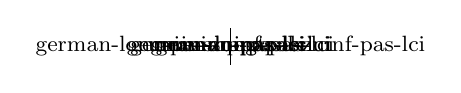
\begin{tikzpicture}[baseline, sibling distance=2pt, level distance=60pt]\footnotesize
		\Tree
		[.{\type{univ-pas-bas-lci}}
		[.\node(D){\type{univ-do-pas-lci}} ;
		[.\node(Z){\type{german-zuinf-pas-lci}} ;
		[.{\type{german-pers-zuinf-pas-lci}} 
		[.\node(PZ){\type{german-long-pers-neutral-zuinf-pas-lci}};
		[.{\type{german-long-pers-zuinf-pas-lci}} ]
		[.{\type{german-long-attr-zuinf-pas-lci}} ]
		]		
		]
		]
		]
		[.\node(G){\type{german-pas-lci}};
		\edge[draw=none]; {}
		[.\node(L){\type{german-long-pas-lci}};
		\edge[draw=none]; {} ]
		{\type{german-io-pas-lci}}	
		]
		\node[sibling distance=-150pt]{\type{univ-imp-pas-lci}} ;
		{\ldots}
		]
		\draw(G.south) -- (Z.north); 
		\draw(L.south) -- (PZ.north);
		\end{tikzpicture}
	}
	\caption{\label{fig:pass-hier}A portion of the hierarchy of passive lexical types according to Ackermann and Webelhuth, p.244}	
\end{figure}


While all passives share the constraint that a logical subject is demoted, as stipulated on a general \type{univ-pas-bas-lci} passive type, the other requirements for each kind of passive are stated on various subtypes.
The \word{zu}+infinitive passive, for instance, requires not only that \word{sein} is the auxiliary and that the main verb is infinitive, but that the semantics involves necessity or obligation.
This differs from the other passives, which simply maintain the semantics of their active counterparts.
However, the types of the passive verb \word{schenken(den)} in (\ref{zu-pass}) both inherit from several passive verb supertypes.
As mentioned, at a general level, there is information common to all German passives, or indeed to passives universally, namely that the ``logical subject'' (first element of the basic verb's \attrib{arg-st} list) is realized as an oblique complement of the passive verb, or not at all.
A very common subtype, which Ackerman \& Webelhuth also regard as universal, rather than specific to German, specifies that the base verb's direct object is realized as the subject of its passive counterpart; this defines personal passives.
Once in the German-specific realm, an additional subtype specifies that the logical subject, if realized, is the object of a \word{von}-PP; this holds true of all three types of German personal passives.
Among its subtypes is one that requires \word{zu} and the infinitive form of the verb; moreover, although Ackerman \& Webelhuth do not spell this out in detail, this subtype specifies the modal force characteristic of this passive construction but not of the others.
Finally, both the predicative and attributive forms are subtypes of all the preceding, but these inherit also from distinct supertypes for predicative and attributive passives of all kinds.
The supertype for predicative passives constrains them to occur with an auxiliary; its subtype for \word{zu} + infinitive passives further specifies that the auxiliary is \word{sein}.
The attributive passive type, on the other hand, inherits from modifier types generally, which do not allow auxiliaries, but do require agreement in person, number, and case with the modified noun.
In summary, the hierarchical lexicon is deployed here to factor out the differing properties of the various German passive constructions, each of which obtains its particular combination of properties via multiple inheritance.

The most specific types of the lexical hierarchy, where individual lexical entries reside, is where constraints pertaining solely to a given word or root -- its phonological form, inflectional class, specific semantics, register, and so forth -- are stated.
Specific information about a word needs to be spelled out somewhere in any grammatical framework.
In a hierarchically organized lexicon we can view this as just the narrowest, most particular case of specifying information about a class of linguistic entities.
But where information is shared across a broader set of lexical entries, it need not be stated separately for each one.
Thus, the phonology of the word \word{spray} and the precise manner of motion of the particles or liquid caused to move in a spraying event are unique to this lexical entry.
However, much of its syntactic and semantic behavior--- it is a regular verb,  participating in a locative alternation, involving caused ballistic motion of a liquid or other dispersable material--- is shared with other English verbs such as \word{splash}, \word{splatter}, \word{inject}, \word{squirt}, and \word{drizzle}.
To the extent that these ``narrow conflation classes,'' as Pinker (1989) terms them, are founded on clear semantic criteria, we can readily state syntactic and semantic constraints at the appropriate level in the hierarchical lexicon (some, however, such as \citet{BriscoeandCopestake1999}, cast doubt on the feasibility of formulating such constraints for dative and other alternations in English, suggesting that lexical rules might be a better alternative).
Given this semantic similarity, it may be that much of the semantics of a verb like \word{spray} need not be specified at the level of that individual lexical entry.
Apart from the broad semantics of caused motion, shared by numerous verbs, the verbs in the narrow conflation class containing \word{spray} share the selectional restriction, noted above, that their objects are set in motion by an initial impulse and that they are liquid or particulate material.
We might therefore posit a subtype of the type \type{caused-motion-rel} to represent this shared semantics triggering the locative alternation, with further subtypes of that for the semantics of the individual verbs.
Note that not all these constraints apply to precisely the same class (there are other verbs with somewhat different semantics, like \word{load} and \word{wrap}, exhibiting the locative alternation, for example), so a multitude of types in the hierarchy is crucial.


\subsection{Default inheritance in the lexicon}

So far, we have assumed rigid, monotonic inheritance of all information in supertypes to their subtypes; none of the inherited information can be overridden.
This runs into difficulties when dealing with lexical entries that appear to be exceptional in some way, the obvious examples being morphological irregularities.
How can productive regular forms such as \word{*childs} be blocked, and only \word{children} allowed as a lexical entry?

While several approaches to exceptions have been proposed, we will focus here on \emph{default unification}; that is, weakening monotonic inheritance in some circumstances.
Then, although the plural of \word{child} might inherit the information from the pertinent lexical entry and from the \type{plural-noun} type, which would entail the phonology for *\word{childs}, this regular plural form is overridden.
Various complex issues arise in attempting to formulate a workable system of default unifcation and inheritance.
See, e.g., \citet{BriscoeandCopestake1999} for a brief overview of various ways that default unification might be defined.
\citet{LC99a} list several desirable criteria, including:

\begin{itemize}
	\item Non-default information is always preserved
	\item Default unification behaves like monotonic unification whenever possible
	\item Default unification is order-independent
\end{itemize}

They explore the properties of their system, called YADU, in considerable detail.
The intent is to preserve the behavior of non-default unification in cases where no default information is present, and for defeasible information at more specific level in the type hierarchy to override defeasible information at a more general level.

As another example of the use of default, nonmonotonic inheritance, outside of morphology, consider the account of the syntax of gerunds in various languages developed by \citet{Malouf2000b}.
Gerunds exhibit both verbal and nominal characteristics, and furnish a well-known example of seemingly graded category membership, which does not accord well with the categorical assumptions of mainstream syntactic frameworks.
Roughly speaking, English gerunds, and their counterparts in other languages, act much like verbs in their ``internal'' syntax, allowing direct objects and adverbial modifiers, but function distributionally (``externally'') as NPs. To take but a couple of pieces of evidence (see Malouf, op.cit. p.27 et seq. for more details), gerunds can be the complement of prepositions when finite clauses cannot (see (\ref{ger-n})); conversely, adverbs, but not adjectives can modify gerunds, but adjectives must modify deverbal nouns (see (\ref{ger-v})).


\begin{exe}
	\ex\label{ger-n}
	\begin{xlist}
		\ex\label{ger-n-a}
		Pat is concerned about Sandy('s) getting arrested.
		\ex\label{ger-n-b}
		*Pat is concerned about (that) Sandy got arrested.
	\end{xlist}	
	\ex\label{ger-v}
	\begin{xlist}
		\ex\label{ger-v-a}
		Pat disapproved of (me/my) *quiet/quietly leaving before anyone noticed.
		\ex\label{ger-v-b}
		Pat disapproved of my quiet/*quietly departure.
	\end{xlist}
\end{exe}



In contrast to accounts that attempt to model this dichotomy directly, via syntactic rules that allow an NP to be expanded as a constituent internally headed by a verb, Malouf posits a lexical rule, which converts the lexical category of a verb to \type{noun}, but otherwise preserves its verbal properties, such as subcategorization.
This would pose problems with strictly monotonic inheritance, however, as it would force us to abandon generalizations about nouns other than gerunds (e.g., they do not take direct object complements, as many verbs and their gerunds do).
Default inheritance provides one way to model the observed phenomena, without weakening the constraints on parts of speech to the point where no meaningful constraints distinguish them. 

Malouf notes that some possible combinations of noun-like and verb-like attributes are frequently attested cross-linguistically in gerunds and their equivalents, while others are rare or unattested.
Cross-linguistically, gerunds vary in their subcategorization possibilities: some allow subjects and complements, while some allow only complements and no subjects.
But there appear to be no cases of gerund-like lexical items that can take a subject but cannot take complements.
Malouf invokes default inheritance \citep{LC99a} as a mechanism to represent these generalizations.
In his account, there are both ``hard'' constraints -- a verb lexical entry, for example, must have a \attrib{head} value of type \type{relational} (encompassing verbs, adjectives, and adpositions) -- and ``soft'', overridable constraints -- a verb lexical entry by default has a \attrib{head} value of type \type{verb}.
In addition, following \citet{Boumaetal2001}, he posits the types \type{ext-subj} and \type{ext-spr}.
The former constrains the \attrib{head} value to \type{relational} and the first element of the \attrib{arg-st} list to be the \attrib{subj} (only adjective, adpositions, and verbs have subjects), while the latter constrains the \attrib{head} value to \type{noun} and the first element of the \attrib{arg-st} list to be the \attrib{spr} (only nouns have specifiers), as shown in (\ref{ext-ss}).


\begin{exe}
	\ex\label{ext-ss}
	\begin{tabular}{llll}
		a. &\begin{avm}
			\[ \asort{ext-subj}
			head & relational \\
			val & \[subj & \@1\] \\
			arg-st & \<\@1, \ldots\> \] 
		\end{avm}
		& b. &
		\begin{avm}
			\[\asort{ext-spr}
			head & noun \\
			val & \[spr & \@1\] \\
			arg-st & \<\@1, \ldots\>\] 
		\end{avm}
	\end{tabular}
\end{exe}

Malouf then specifies default \attrib{head} values for the lexical classes \type{n} and \type{v} (see (\ref{v-def}) for the latter's definition). As gerunds have both properties of nominal and relational heads, they are subtypes of both, as shown in the multiple inheritance hierarchy in (\ref{ger-hier}). The \type{v} type, which concerns us here, has a default \attrib{head} value \type{verb}, as shown in (\ref{v-def}) in addition to the non-default, more general type \type{relational} it also includes (default information follows $/$).


\begin{exe}
	\ex\label{ger-hier}
	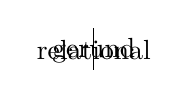
\begin{tikzpicture}[baseline]
	\Tree
	[.{\type{head}}
	[.{\type{func}} {\type{det}} {\type{marker}} ]
	[.{\type{subst}} [.{\type{noun}} 
	{\type{c-noun}} \node(G){\type{gerund}}; 
	]
	[.\node(R){\type{relational}};
	\edge[draw=none]; {}
	{\type{verb}} {\type{adj}} {\type{prep}}
	] ]
	]
	\draw(R.south) -- (G.north);
	\end{tikzpicture}
\end{exe}


\begin{exe}
	\ex\label{v-def}
	\begin{avm}
		\[\asort{v}
		head & relational /verb \\
		cont & psoa \]
	\end{avm}
\end{exe}


However, the default value \type{verb} is overridden in the subtype \type{vger}, in which the \attrib{head} value is \type{gerund}, which is a subtype of both \type{noun} and \type{relational}, but not of \type{verb}.
The type \type{vger} is shown in (\ref{vger}); where \type{f-ing} is a function the produces the \word{-ing} form of an English verb from its root.


\begin{exe}
	\ex\label{vger}
	\begin{avm}
		\[\asort{vger}
		morph & \[
		root & \@1 \\
		i-form & f-ing(\@1) \]\\
		head & gerund \]
	\end{avm}
\end{exe}


The type \type{vger} is thus compatible with ``verb-like'' characteristics; in particular, it has an \attrib{arg-st} list.
But, as its \attrib{head} is also a subtype of \type{noun}, it lacks a \attrib{subj} attribute and instead has a \attrib{spr} attribute.
Gerunds therefore allow complements (unlike ordinary nouns), but not subjects (unlike ordinary verbs).
Malouf's hierarchy of types makes this prediction, in effect, because the \type{ext-spr} type requires that the ``external argument'' (the first on the \attrib{arg-st} list) is realized as the value of\attrib{spr}.

While it would be possible to construct type hierarchies of lexical types, \attrib{head} types, and so on that would allow for this kind of ``reverse gerunds'' -- those that would act externally as nouns, allow subjects, but not permit complements -- this would require reorganizing these type hierarchies to a considerable extent.
Given that many nouns besides gerunds -- nominalizations, for example -- are relational (that is, have a \attrib{content} value of type \type{psoa}), it could be difficult to model a hypothetical language that permits only the reverse gerunds rather than the normal ones.

Malouf further notes a key difference between gerunds and exceptions like *\word{childs}/\word{children}: English gerunds are productive (and completely regular morphologically).
If the same mechanisms of default unification are involved in both, what accounts for this difference?
His answer is that productive and predictable processes involve online type construction (see Section \ref{sec:alt} for details).
The irregular form \word{children} must of course be learned and stored, not generated online.
The default mechanisms described above, however, are employed at higher levels of the lexical hierarchy, and the individual gerunds forms \emph{are} productively generated online.
Note that, in contrast to the morphological and syntactic consistency among gerunds, English nominalizations display some idiosycrasies that suggest at least some of them must be stored as distinct lexical items.
Thus, as Malouf emphasizes, modeling prototypicality in the lexicon within HPSG can draw on both default inheritance and online type construction; together, they make ``the connection between prototypicality, and productivity.''



\section{Lexical rules}

In this section we describe the role lexical rules play in HPSG as well as their formal nature, i.e., how they model ``horizontal'' relations among elements of the lexicon. These are relations between variants of a single entry (be they subcategorizational or inflectional variants) or between members of a morphological family, as opposed to the ``vertical'' relations modeled through inheritance. Thus they provide a means to represent the intuitive notion of ``derivation'' of one lexeme from another. 

While lexical rules or similar devices have been invoked within HPSG since its inception, formalizing their nature and behavior was deferred until somewhat later. 
The intent, however, has always been, as \citet{Lahm2016} stresses, to treat lexical rules (typically written $A \mapsto B$) to mean that for every lexeme or word described by $A$ there is one described by $B$ that has as much in common with A as possible.

\citet{CopestakeandBriscoe1991}, \citet{BriscoeandCopestake1999}, \citet{Meurers2001}, and many others formalize the notion of lexical rule within HPSG by introducing a type, say \type{lex-rule}, with the attributes \attrib{in} and \attrib{out}, whose values are respectively the rule's input and output lexical entries. As \citet{BriscoeandCopestake1999} note, lexical rules of this form also bear a close relationship to default unification.
The information in the input is intended to carry over to the output by default, except where the rule specifies otherwise and overrides this information. But, as \citet{Lahm2016} points out, a sound basis for the formal details of how lexical rules work is not easy. Meurers' careful analysis of how to apply lexical rules to map a description of an entry $A$ into the description $B$ does not always work as intended in that what would expect to be licit inputs are actually not and no output description results as a consequence. Fortunately,  it is not clear that this is a severe problem in practice, and Lahm notes that he has not found an example of practical import where Meurers's lexical rule formulation would encounter the problems he raises.

In a slight variant of the representation of lexical rules proposed by Copestake \& Briscoe and Meurers, the \attrib{out} attribute can be dispensed with; the information in the lexical rule type not within the \attrib{in} value then constitutes the output of the rule.
In this variant, lexical rules could alternatively be viewed as be subtypes of a \type{derived-word} type, which could combine with other types in the lexical hierarchy, merely adding the derivational source via the \attrib{in} value. 
Formulated in either fashion, lexical rules are essentially equivalent to unary syntactic rules, with the \attrib{in} attribute corresponding to the daugther and the \attrib{out} attribute (or the rest of the information in the rule, if the \attrib{out} attribute is done away with) to the mother. This is the way lexical rules are implemented in the English Resource Grammar (see \url{http://www.delph-in.net/erg/} for demos and details about this large-scale implemented grammar of English). (cross-reference to Bender \& Emerson's chapter on computational linguistics and language engineering here)


\subsection{Phenomena accounted for by lexical rules}

Lexical rules have been put to many uses, derivational and inflectional morphology \citep{CopestakeandBriscoe1995,EmersonandCopestake2015}, complex predicate formation \citep{MuellerPersian}, and diathesis alternations \citep{Davis2001}. Moreover, proposals for lexical rules in HPSG have extended beyond what are traditionally or evidently viewed as lexical phenomena, to include treatments of extraction, unbounded dependencies, and adjuncts. In this section, we describe the use of lexical rules to model the realization of arguments as extracted dependents or affixes, rather than complements. We concentrate on these two cases, which we will contrast with alternative analyses not involving lexical rules presented by the same authors (see the next section). They thus provide a good illustration of some of the analytical choices available to model relations between variant lexical entries that are based on a single stem. 


We begin with the Complement Extraction Lexical Rule (hereafter, CELR) proposed in \citew{PollardandSag1994} shown in (\ref{celr}). The input to the rule is any lexeme that selects for a syntactic argument (\avmbox{3}) that the lexeme requires be expressed as a complement (as indicated, this syntactic argument is also a member of the \attrib{comps} list). The ouput stipulates that this same syntactic argument is no longer a member of the \attrib{comps} list; however, the \attrib{slash} set now includes a new element, which is the local information of this syntactic argument (\avmbox{1}). Informally stated, the input entry specifies that a syntactic argument must be realized as a complement, whereas the output entry specifies that the same syntactic argument must be realized by a non-local dependent (see \citet{PollardandSag1994} for why only \attrib{local} information is shared between syntactic arguments and fillers that realize them).

\begin{exe}
	\ex\label{celr}
	\begin{avm}
		\[arg-st & \< \ldots, \@3, \ldots \>\\
		comps & \<\ldots,\@3\[loc & \@1\], \ldots \>\\
		slash & \@2
		\]
	\end{avm}
	$\mapsto$
	\begin{avm}
		\[arg-st & \< \ldots, \@4\[loc \@1\\ slash & \@1\], \ldots \>\\
		comps & \<\ldots \>\\
		slash & \{ \@1\} $\cup$ \@2
		\]
	\end{avm}
\end{exe}


A similar use of lexical rules to model alternative realizations of arguments can be found in \citew{Monachesi1993}, who analyzes alternations between complements and so-called object clitics in Italian in a way that parallels the French examples in (\ref{va}). In the output of her lexical rule, in (\ref{cl-lr}), a subset of the list of complements in the input (\avmbox{2}) corresponds to a list of clitic \attrib{synsem}s, realized as prefixes through inflectional rules not shown here.

\begin{exe}
	\ex\label{cl-lr}
	\begin{avm}
		\[\asort{word}
		head & verb \\
		val$|$comps & \@1 $\bigcirc$ \@2 \\
		clts & elist
		\]
	\end{avm}
	$\mapsto$
	\begin{avm}
		\[\asort{word}
		val$|$comps & \@1  \\
		clts & \@2list(cl-ss)
		\]
	\end{avm}
\end{exe}

Here as well, a lexical rule is employed in an analysis of what might well be considered a syntactic phenomenon.
The possibility of treating phenomena like extraction and clitic placement at a lexical level, however, makes sense when they are considered fundamentally as matters of the combinatorial requirements of predicators, rather than effects of movement.

Before turning to the alternatives, we note in passing that lexical rules are inherently ``directional'', with an input and an output.
This seems intuitively correct in the cases we've discussed, but might not always be so.
Is there inherent directionality, for example between the causative and inchoative alternants of verbs such as \word{melt} or \word{slide}?
In constrast, the alternatives to lexical rules described in the following section lack this notion of directionality.


\subsection{Alternatives to lexical rules}
\label{sec:alt}

In this section we briefly examine two alternatives to lexical rules, each involving underspecification. The types of members of the \attrib{arg-st} list might be underspecified so that a lexical entry accounts for more than one subcategorization. Or the type of the entry itself may be underspecified, so that it subsumes multiple inflectional or derivations forms. In both cases, the intent is that sufficiently underspecified information covers multiple entries that would otherwise have to be specified and related by lexical rules. We begin with alternatives to the complement extraction and clitic lexical rules in (\ref{celr}) and (\ref{cl-lr}), proposed in \citew{Boumaetal2001} and \citew{MillerandSag1997}. 

In both cases, the idea is to distinguish between ``canonical'' and ``non-canonical'' realizations of syntactic arguments, as shown in the hierarchy of \type{synsem}s in (\ref{synsem}). ``Canonical'' means local realization as a complement or subject/specifier, and ``non-canonical'' means realization as an affix or filler of an unbounded dependency. Linking constraints between semantic roles (values of argument positions) and syntactic arguments (members of \attrib{arg-st}) do not specify whether the realization is canonical or not; thus they retain their original form. Only canonical members of \attrib{arg-st} must be structured-shared with members of valence lists. The two constraints that determine the non-canonical realization of fillers are shown in (\ref{fillers}). (\ref{gap}) specifies what it means to be a \type{gap-ss}), namely that the argument is extracted (its local information is ``slashed,'') whereras (\ref{wd-bouma}) prohibits any \type{gap-ss} member from being a member of the \attrib{comps} list. As these two constraints are compatible with either a canonical or extracted object, there is no need for the lexical rule is (\ref{celr}).

\begin{exe}
	\ex\label{synsem} \Tree
	[.{\type{synsem}} \type{canon-ss} [.{\type{non-canon-ss}} {\type{gap-ss}} 
	{\type{aff-ss}} ] ]	
\end{exe}

\begin{exe}
	\ex\label{fillers}
	\begin{xlist}
		\ex\label{gap}
		\type{gap-ss} $\Rightarrow$
		\begin{avm}
			\[loc & \@1 \\
			slash & \@1 \]
		\end{avm}
		\ex\label{wd-bouma}
		\type{word} $\Rightarrow$
		\begin{avm}
			\[subj & \@1 \\
			comps & \@2$\ominus$list(gap-ss) \\
			deps & \@1 $\oplus$ \@2
			\]
		\end{avm}
	\end{xlist}
\end{exe}

\citet{MillerandSag1997} make a similar use of non-canonical relations between the \attrib{arg-st} list and the valence lists, eschewing lexical rules to model French clitics and proposing instead the constraint in (\ref{cl-wd}), where a subset of \attrib{arg-st} members, those that are realized as affixes (of type \type{aff}) are not also subcategorized for as complements. 

\begin{exe}
	\ex\label{cl-wd}
	\begin{avm}
		\[morph & \[form & F$_{PRAF}$(\@1, \ldots) \\
		i-form \@1 \] \\
		synsem & \[loc$|$cat & \[head & verb \\
		val & \[subj & \@2 \\
		comps & 
		\@3list(non-aff) \] \\
		arg-st & $($\@2$\oplus$\@3$)$ $\bigcirc$ nelist(aff)\]\]\]
	\end{avm}
\end{exe} 



The second alternative to lexical rules based on underspecification was presented in \citew{KoenigandJurafsky1994} and \citew{Koenig99a}. Typically in HPSG, all possible combinations of types are reified in the type hierarchy (in fact, they must be present, per the requirement that the hierarchy be sort-resolved, \citealt{Carpenter92a},\citealt{PollardandSag1994}). Thus, if one partitions verb lexemes into transitive and intransitive and, orthogonally, into, say, finite verbs and gerunds (limiting ourselves to two dimensions here for simplicity), the type hierarchy must also contain the combinations transitive+finite, transitive+gerund, intransitive+finite, and intransitive+gerund. Naturally, this kind of fully enumerated type system is unsatisfying. For one thing, there is no additional information that the combination subtype transitive+finite carries that is not present in its the two supertypes transitive and finite, and similarly for the other combinations. In contrast to the ``ordinary'' types, posited to represent information shared by classes of lexemes, these combinations seem to have no other function than to satisfy a formal requirement of the mathematical structure of a type hierarchy (namely, that it forms a lattice under meet and join).  Second, and related to the first point, this completely elaborated type hierarchy is redundant. Once you know that all verbs fall into two valence classes, transitive and intransitive, and simultaneously into two inflectional classes, finite and gerund, and that valence and inflection are two orthogonal dimensions of classification of verbs, you know all you need to know; the type of any verb can be completely predicted from these two orthogonal dimensions of classification and standard propositional calculus inferences.

In (\ref{verb-hier2}) is a simplified version of the hierarchy in (\ref{verb-hier}), where the boxed labels in small caps \attrib{vform} and \attrib{arg-st} are mnemonic names of orthogonal dimensions of classification  of subcategories of verbs (and are not themselves labels of subcategories). Inheritance links to the predictable subtypes are dashed and their names grayed out; this indicates that these types can be inferred, and need not be declared explicitly as part of the grammar. A grammar of English would include statements to the effect that head information about verbs includes a classification of verbs into finite or base forms (of course, there would be more types of verb forms in a realistic grammar of English) as well a classification into intransitive and transitive verbs (again, a realistic grammar would include many more types).


\begin{exe}
	\ex\label{verb-hier2}
	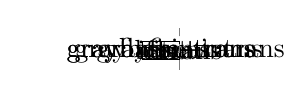
\begin{tikzpicture}[baseline]
	\Tree
	[.{\type{verb}} 
	[.{\fbox{\attrib{vform}}}
	[.\node(A1)  {\type{fin}};  
	\edge[dashed,gray]; [.\node(A) {\tc{gray}{\type{fin+intrans}}}; ]     			
	\edge[draw=none]; {} ]
	[.\node(B1) {\type{base}}; 
	\edge[dashed,gray]; [.\node(B){\tc{gray}{\type{base+trans}}};  ]   		 
	\edge[draw=none]; {} ]
	]
	[.{\fbox{\attrib{arg-st}}} 
	[.\node(C1) {\type{intrans}} ; 
	\edge[draw=none]; {} 
	\edge[dashed,gray]; [.\node(C) {\tc{gray}{\type{base+intrans}}};  ] ]
	[.\node(D1) {\type{trans}}; 
	\edge[draw=none]; {}  
	\edge[dashed,gray]; [.\node(D) {\tc{gray}{\type{fin+trans}}}; ]   ]
	]  
	]
	\draw[style=dashed,gray] (C1.south) -- (A.north);
	\draw[style=dashed,gray] (D1.south)-- (B.north);
	\draw[style=dashed,gray] (B1.south)-- (C.north);
	\draw[style=dashed,gray] (A1.south)-- (D.north);
	\end{tikzpicture}
\end{exe}

\citet{CrysmannandBonami2016} have shown how this \word{online type construction}, where predictable combinations of types of orthogonal dimensions of classification are not reified in the grammar, is useful when modeling productive inflectional morphology. Consider, for example, exponents of morphosyntactic features whose shape remains constant, but whose position within a word's template (to speak informally here) varies. One case like this is the subject and object markers of Swahili, which can occur in multiple slots in the Swahili verb template. For reasons of space we illustrate the usefulness of this dynamic approach to type creation, the Type Underspecified Hierarchical Lexicon (\attrib{tuhl}) with an example from \citet{Koenig99a}, the cross-cutting classification of syntactic/semantic information and stem form in the entry for the French verb \word{aller} (see \citet{BonamiandBoye2001} for a much more thorough discussion of French stem allomorphy along similar lines; Crysmann and Bonami's much more developed approach to stem allomorphy would model the same phenomena differently and we use Koenig's simplified presentation for expository purposes only). The forms of \word{aller} are based on four different suppletive stems: \word{all-} (1\textsuperscript{st} and 2\textsuperscript{nd} person plural of the indicative and imperative present, infinitive, past participle, and imperfective past), \word{i-} (future and conditional), \word{v-} (1\textsuperscript{st}-3\textsuperscript{rd} person singular and 3\textsuperscript{rd} person plural of the indicative present), and \word{aill-} (subjunctive present). These four suppletive stems are shared by all entries (i.e., senses) of the lexeme \word{aller}: the one which means `to fit' as well as the one which means `to leave', as shown in (\ref{aller-lex}) (see Koenig, op.cit, p.40-41). The cross-cutting generalizations over lexemes and stems are represented in Figure \ref{all-hier}. Any \word{aller} stem combines one entry and one stem form. In a traditional HPSG type hierarchy, each combination of types (grayed out in Figure \ref{all-hier}), would have to be stipulated. In a \attrib{tuhl}, these combinations can be dynamically created when an instance of \word{aller} needs to be produced or comprehended.

\begin{exe}
	\ex\label{aller-lex}
	\begin{xlist}
		\ex\label{aller-lex-a}
		\gll Marc est allé à Paris. \\
		Marc be-\ig{pr.3rd.sg} go-\ig{ppt} to Paris \\
		\glt `Marc went to Paris.'
		\ex\label{aller-lex-b}
		\gll Marc s'en ira. \\
		Marc \ig{3.refl}-of.it go-\ig{fut.3rd.sg} \\
		`Marc will leave.'
		\ex\label{aller-lex-c}
		\gll Ce costume te va bien. \\
		This suit you go-\ig{pr.3.sg} well \\
		\glt `This suit becomes you.' (lit. goes well to you)
		\ex\label{aller-lex-d}
		\gll Il faut que j'y aille. \\
		It must that I.to.there go-\ig{subj.pr.1.sg} \\
		\glt `I must go there.'
	\end{xlist}	
\end{exe}


\begin{sidewaysfigure}
	\oneline{%
		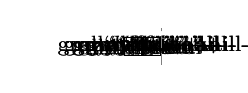
\begin{tikzpicture}[baseline]\footnotesize
		\tikzset{level 1/.style={level distance=50pt}}
		\tikzset{level 2/.style={level distance=50pt}}
		\tikzset{frontier/.style={distance from root=280pt}}
		\Tree
		[.{\type{aller}}
		[.{\fbox{\type{aller-entries}}}
		[.\node(F){\type{aller-``fit}};
		\edge[dashed,gray]; \node(F1){\tc{gray}{\type{``fit''+all-}}};
		\edge[dashed,gray]; \node(F2){\tc{gray}{\type{``fit''+v-}}};
		\edge[draw=none]; {} 
		\edge[draw=none]; {} ]
		[.{\type{aller-``go''}}
		[.\node(G){\type{aller-``go.to''}};
		\edge[dashed,gray]; \node(G1){\tc{gray}{\type{``go.to''+all-}}};
		\edge[dashed,gray]; \node(G2){\tc{gray}{\type{``go.to''+v-}}};
		\edge[draw=none]; {}
		\edge[draw=none]; {} ]
		[.\node(L){\type{aller-``leave''}};
		\edge[dashed,gray]; \node(L1){\tc{gray}{\type{``leave''+all-}}};
		\edge[dashed,gray]; \node(L2){\tc{gray}{\type{``leave''+v-}}};
		\edge[draw=none]; {}
		\edge[draw=none]; {}
		]]
		]
		[.{\fbox{\type{aller-stems}}}
		[.\node(A){\type{all-stem}};
		\edge[draw=none]; {}
		\edge[draw=none]; {}
		\edge[draw=none]; {}
		]
		[.\node(V){\type{v-stem}};
		\edge[draw=none]; {}
		\edge[draw=none]; {}
		\edge[draw=none]; {}
		]
		[.\node(I){\type{i-stem}};
		\edge[dashed,gray]; \node(I1){\tc{gray}{\type{``fit''+i-}}};
		\edge[dashed,gray]; \node(I2){\tc{gray}{\type{``go.to''+i-}}};
		\edge[dashed,gray]; \node(I3){\tc{gray}{\type{``leave''+i-}}};
		]
		[.\node(AI){\type{aill-}};
		\edge[dashed,gray]; \node(A1){\tc{gray}{\type{``fit''+aill-}}};
		\edge[dashed,gray]; \node(A2){\tc{gray}{\type{``go.to''+aill-}}};
		\edge[dashed,gray]; \node(A3){\tc{gray}{\type{``leave''+aill-}}};  	]
		]
		]
		\draw[style=dashed,gray](A.south) -- (F1.north); 
		\draw[style=dashed,gray](V.south) -- (F2.north); 
		\draw[style=dashed,gray](A.south) -- (G1.north); 
		\draw[style=dashed,gray](V.south) -- (G2.north); 
		\draw[style=dashed,gray](A.south) -- (L1.north); 
		\draw[style=dashed,gray](V.south) -- (L2.north); 
		\draw[style=dashed,gray](F.south) -- (I1.north);
		\draw[style=dashed,gray](F.south) -- (A1.north);
		\draw[style=dashed,gray](G.south) -- (I2.north);
		\draw[style=dashed,gray](G.south) -- (A2.north);
		\draw[style=dashed,gray](L.south) -- (I3.north);
		\draw[style=dashed,gray](L.south) -- (A3.north);
		\end{tikzpicture}}
	\caption{\label{all-hier} A hierarchy of lexical entries and stem-forms for the French verb \word{aller}, from \citew{Koenig99a}}
\end{sidewaysfigure}



\pagebreak


Both \type{synsem} and type underspecification avoid conflict between the information specified in the variants of words based on a single lexeme (e.g., conflicts on how syntactic arguments are realized); they abstract over the relevant pieces of conflicting information. Underspecifying information included in lexical entries or lexical types allows a single entry or type to stand for the two distinct entries or types that would be related as input and output by lexical rules. The third alternative to lexical rules eschews informational conflict by adding internal structure to stems and words. This is the approach to derivational morphology taken by \citet{Riehemann1998}. Example (\ref{bar}) (Riehemann's (1)) illustrates \word{-bar} suffixation in German, a process by which an adjective that includes a modal component can be derived from verb stems (similar to English \word{-able} suffixation). A lexical rule approach would posit a verb stem input and derive an adjective output. As Riehemann stresses, though, there are many different subtypes of \word{-bar} suffixation, some productive, some unproductive, all sharing some information. This combination of productive and unproductive variants of a lexical process is exactly what the type hierarchy is meant to capture and what Riehemann's \word{Type-Based Derivational Morphology} capitalizes on. (\ref{bar-der}) presents the relevant information of Riehemann's type for regular \word{-bar} adjectives (see p.68 for more details). Critically, \word{-bar} adjectives include a singleton-list base (the value of \attrib{morph-b}) that records the information of the adjective's verbal base (what would be the lexical rule's input). Because of this extra layer, the local information in the base (\type{local${1}$}) and the \word{-bar} adjective (\type{local$_{2}$}) can differ without being in conflict.

\begin{exe}
	\ex\label{bar}
	\gll Sie bemerken die Ver\"anderung. Die Ver\"anderung ist bemerkbar. \\
	They notice the change. The change is noticeable. \\
\end{exe}    

\begin{exe}
	\ex\label{bar-der}
	\begin{avm}
		\[\asort{reg-bar-adj}
		phonology & \@1+bar \\
		morph-b & \<\[\asort{trans-verb}
		phon & \@1 \\
		local & local$_{1}$ \]\> \\
		synsem$|$local & local$_{2}$ \]					
	\end{avm}
	
\end{exe}

Lexical rules played a critical role in the rise of lexicalist approaches to syntax. But the three alternative analytical tools we discussed in this section (which, of course, can be combined in an analysis) have chipped away at their use in HPSG. Inflectional morphology is now dealt with through lexical types associating morphosyntactic features with forms/positions and constraints on words (ensuring that all morphosyntactic features are realized). (cross-reference the chapter on Morphology)
Derivational morphology is handled via lexical types too, but ones that add an extra internal layer (the \attrib{morph-b}ase in Riehemann's analysis and (\ref{bar-der})). 
Non-canonical realization of syntactic arguments as affixes or fillers in unbounded dependencies is now modeled by distinguishing kinds of members of the \attrib{arg-st} list and constraints on words that relate valence, argument structure, and dependents lists. So, what remains of the case for lexical rules now? \citet{Mueller2006,MuellerPersian} argues that diathesis phenomena, broadly speaking, favor a lexical rules approach over a phrase-structural constructional approach à la \citet{Goldberg95a} or an online type construction approach suggested in \citew{Kay2002}. The arguments are convincing, but it should be noted that some of the data involves derivational morphology (e.g., causatives) or passive morphemes, which, arguably, could be handled via a Type-Based Derivational Morphology of the kind Riehemann argues for (such an approach was suggested in \citet[Chapter~4]{Koenig99a}). 
It is unclear to us whether there are always motivated types for morphologically derived stems to dispense entirely with lexical rules of the kind Müller argues for. On the other hand, if one adopts the version of lexical rules in which the \attrib{out} attribute is eliminated and lexical rules are subtypes of \type{derived-lexeme}, little will be at stake formally, as lexical rules and derivational processes ``look the same.'' 




 
\section*{Abbreviations}
\section*{Acknowledgements}

{\sloppy 
\printbibliography[heading=subbibliography,notkeyword=this] 
}

\end{document}
